\RequirePackage{import}
\subimport{../../exercises}{preamble.tex}

% Packages
\usepackage{hyperref}

%\usepackage{ClearSans}
\usepackage{csquotes}
\usepackage{tikz}
\usetikzlibrary{fit,backgrounds}


\usepackage[font=normalsize, labelfont=sf, position=bottom]{caption}
\usepackage[labelfont=normalfont, position=bottom]{subcaption}
% Stylistic Changes
\captionsetup[figure]{justification=centering}
\setlength{\parindent}{0pt}

\def\gamefont{\bfseries\sffamily}
%
\definecolor{grid color}{RGB}{187, 173, 160}
\definecolor{tile 0}{HTML}{CCC0B3}
\definecolor{tile 2}{HTML}{EEE4DA}
\definecolor{tile 4}{HTML}{EEE1C9}
\definecolor{tile 8}{HTML}{F3B27A}
\definecolor{tile 16}{HTML}{F69664}
\definecolor{tile 32}{HTML}{F77C5F}
\definecolor{tile 64}{HTML}{F75F3B}
\definecolor{tile 128}{HTML}{EDD073}
\definecolor{tile 256}{HTML}{EDCC62}
\definecolor{tile 512}{HTML}{EDC950}
\definecolor{tile 1024}{HTML}{EDC53F}
\definecolor{tile 2048}{HTML}{EDC22E}
\definecolor{tile 4096}{HTML}{3C3A33}
%
\definecolor{small color}{HTML}{776E65}
\definecolor{big color}{HTML}{F9F6F2}
%
\tikzset{
    case 2048 base/.style={
        minimum size=9mm,rounded corners=.3mm,text=#1,inner sep=0,line width=0,
    },
    %
    case 2048 Large/.style={font=\Large\gamefont,case 2048 base=#1},
    case 2048 large/.style={font=\large\gamefont,case 2048 base=#1},
    case 2048 normal/.style={font=\normalsize\gamefont,case 2048 base=#1},
    %
    case 2048 0/.style={case 2048 Large=black,fill=tile 0,node contents={}},
    case 2048 2/.style={case 2048 Large=small color,fill=tile 2,node contents={2}},
    case 2048 4/.style={case 2048 Large=small color,fill=tile 4,node contents={4}},
    case 2048 8/.style={case 2048 Large=big color,fill=tile 8,node contents={8}},
    case 2048 16/.style={case 2048 Large=big color,fill=tile 16,node contents={16}},
    case 2048 32/.style={case 2048 Large=big color,fill=tile 32,node contents={32}},
    case 2048 64/.style={case 2048 Large=big color,fill=tile 64,node contents={64}},
    case 2048 128/.style={case 2048 large=big color,fill=tile 128,node contents={128}},
    case 2048 256/.style={case 2048 large=big color,fill=tile 256,node contents={256}},
    case 2048 512/.style={case 2048 large=big color,fill=tile 512,node contents={512}},
    case 2048 1024/.style={case 2048 normal=big color,fill=tile 1024,node contents={1024}},
    case 2048 2048/.style={case 2048 normal=big color,fill=tile 2048,node contents={2048}},
    case 2048 4096/.style={case 2048 normal=big color,fill=tile 4096,node contents={4096}},
}

% Document

\begin{document}


\title{Programmierchallenge Wintersemester 2021/22 \\ {\small der Fachschaft Informatik}}
\subtitle{Wintersemester 2021/22}
\author{Autor: Ruben Deisenroth}
\maketitle

\section*{2048 \hyperref[footnote:1]{\footnotemark[1]}}
\footnotetext[1]{\label{footnote:1}\url{https://de.wikipedia.org/wiki/2048}}
\subsection*{Ablauf des Spiels}
\vspace{-1ex}
\begin{minipage}[t]{.7\textwidth}
    \subsubsection*{Spielbetrieb}
    Zunächst wird ein 4x4 Spielfeld generiert. Dieses Spielfeld kann Felder mit Zweierpotenzen bis $2^{11}$ enthalten
    (also
    \ExplSyntaxOn
    \def\nextsep{}
    \int_step_inline:nnnn {1}{1}{11} {
        \nextsep{}
        \fp_to_int:n {2^#1}\def\nextsep{,~}
    }
    \ExplSyntaxOff
    )

    \smallskip
    Zu Beginn des Spieles werden zwei zufällige, unterschiedliche Felder auf $2$ oder $4$ gesetzt.

    \smallskip
    Der*die Spieler*in kann dann eine Richtung auswählen, in die geschoben wird $(\leftarrow,\rightarrow,\uparrow,\downarrow)$.
    Alle Kacheln verschieben sich dann so weit wie möglich in die gewählte Richtung, also bis sie entweder auf den Rand oder ein anderes gefülltes Feld stoßen.

    \smallskip
    Sollte ein Feld an ein weiteres Feld in Schieberichtung stoßen, welches den gleichen Wert hat, so verschmelzen beide Felder zu einem Feld mit der nächsthöheren Zweierpotenz und werden so weit wie möglich in die Schieberichtung geschoben.
\end{minipage}%
\begin{minipage}[t]{.3\textwidth}%
    \centering%
    \captionsetup{type=figure}
    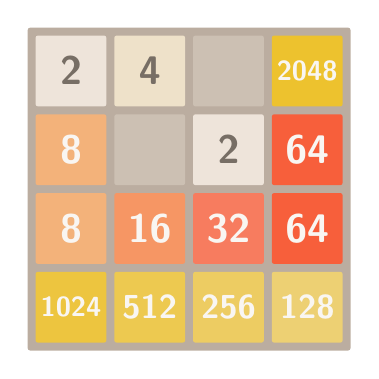
\begin{tikzpicture}
        \def\tiles{
            {2,4,0,2048},
            {8,0,2,64},
            {8,16,32,64},
            {1024,512,256,128},
        }

        \foreach \line [count=\y] in \tiles {
            \foreach \pix [count=\x] in \line {
                \path (\x,-\y) node[name=c2048-\x-\y,case 2048 \pix];
            }
        }

        \begin{scope}[on background layer]
            \node[fill=grid color,fit=(c2048-1-1)(c2048-4-4),
                inner sep=1mm,rounded corners=.3mm]{};
        \end{scope}
    \end{tikzpicture}
    \captionof{figure}{Beispiel 2048}
\end{minipage}%

In jeder weiteren Runde wird ein weiteres, zufälliges, freies Feld mit $2$ oder $4$ gefüllt, und anschließend kann der Spieler wieder eine Schieberichtung auswählen.

\textit{Für Bastler(keineswegs erforderlich):} Die Wahrscheinlichkeit, dass einem freien Feld eine $4$ statt einer $2$ zugewiesen wird, beträgt $10\%$
\vspace{-1ex}
\subsubsection*{Spielende}
Wenn alle Verschiebungsrichtungen zu keiner Änderung führen, und das Spielfeld voll ist, dann ist das Spiel verloren.

Wenn eine Kachel den Wert $2048$ erreicht ist das Spiel gewonnen :D
\vspace{-1ex}
\subsubsection*{Sonderfälle}

Wenn zwei Felder verschmolzen sind, können sie in dieser Runde nicht weiter verschmelzen:

\begin{center}
    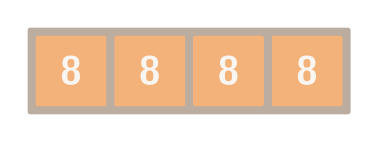
\begin{tikzpicture}[baseline={([yshift=-.8ex]current bounding box.center)}]
        \def\tiles{
            {8,8,8,8},
        }

        \foreach \line [count=\y] in \tiles {
            \foreach \pix [count=\x] in \line {
                \path (\x,-\y) node[name=c2048-\x-\y,case 2048 \pix];
            }
        }

        \begin{scope}[on background layer]
            \node[fill=grid color,fit=(c2048-1-1)(c2048-4-1),
                inner sep=1mm,rounded corners=.3mm]{};
        \end{scope}
    \end{tikzpicture}
    $\stackrel{schieben(r)}{\Longrightarrow}$
    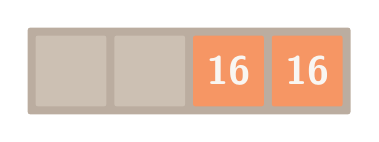
\begin{tikzpicture}[baseline={([yshift=-.8ex]current bounding box.center)}]
        \def\tiles{
            {0,0,16,16},
        }

        \foreach \line [count=\y] in \tiles {
            \foreach \pix [count=\x] in \line {
                \path (\x,-\y) node[name=c2048-\x-\y,case 2048 \pix];
            }
        }

        \begin{scope}[on background layer]
            \node[fill=grid color,fit=(c2048-1-1)(c2048-4-1),
                inner sep=1mm,rounded corners=.3mm]{};
        \end{scope}
    \end{tikzpicture}
\end{center}

Beim Schieben in eine Richtung ist es möglich, dass \enquote{nichts passiert}.
Es wird trotzdem ganz normal als Zug gewertet, und eine neue Runde eingeleitet.


\section*{Das Spiel}
\subsection*{Die Aufgabe}
Programmiert in Python eine Spieladaption des oben beschriebenen $2048$.
Dieses soll auf und in der Konsole funktionieren.
Hierbei soll das Spielfeld nach jedem Zug neu angezeigt werden.
Bei jedem Zug muss der*die Spieler*in mittels der Konsole eine Schieberichtung auswählen, welche die Kacheln verschiebt.

Das Programm soll selbst erkennen wann das Spiel für eine*n der Spieler*innen gewonnen oder verloren ist.
Im Anschluss zeigt das Programm den Ausgang des Spiels an und beendet sich.

\subsection*{Rahmen}
Es existiert kein \enquote{Rahmen} oder \enquote{Framework}.
Das Projekt besitzt außer diesem Dokument keine weiteren Unterlagen.
Bei Fragen könnt ihr euch am besten an die Tutor*innen oder an die Orga wenden.
Bitte haltet euch an das KISS-Prinzip\footnote[2]{\url{https://de.wikipedia.org/wiki/KISS-Prinzip}} (Keep it simple, stupid), versucht also eine möglichst einfache Lösung zu erstellen.
Es muss auch kein Wunderwerk der Technik sein.
Dennoch sind kreative Ideen gerne gesehen.

\subsection*{Die Abgabe}
Es gibt zwei Möglichkeiten der Abgabe: Bis spätestens 23:59 Uhr am Freitag (08.10.2021) könnt ihr eure \texttt{.py}-Datei in Moodle hochladen oder ihr schickt uns eine Mail an \href{mailto:vorkurs@d120.de}{\nolinkurl{vorkurs@d120.de}}.
Dort hängt ihr die Datei bitte als Anhang an.
Dabei gilt die Ankunftszeit bei uns.
\end{document}
